\section{Introduction}
\label{sec:intro}

The Transformer architecture has become the primary backbone for large language models (LLMs), prominently featuring attention mechanism~\cite{vaswani2017transformer} as its most salient component. As LLMs rapidly evolve and find applications in diverse fields, the demand for efficient GPU attention kernels grows, with the goal of enabling scalable and responsive model inference. At the heart of LLM inference lies the attention computation, which plays a crucial role in processing historical context and generating outputs based on query vectors. In LLM serving, the attention mechanism reads from the KV cache, which stores historical context, and computes outputs based on the current query. The efficiency of this attention operator is paramount to the overall performance of an LLM inference systems. However, creating high-performance attention kernels tailored for LLM serving introduces challenges not typically encountered in traditional training environments.

\begin{figure*}[t!]
    \centering
    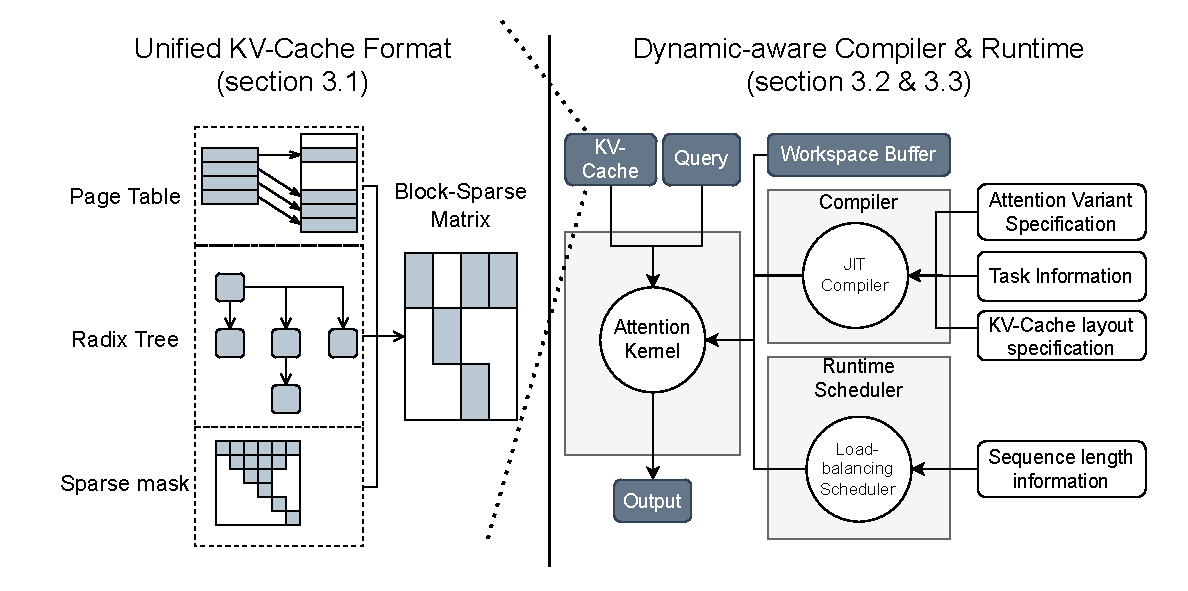
\includegraphics[width=0.85\textwidth]{figures/flashinfer-overview.pdf}
    \caption{Overview of the \sys system design: Attention variant specifications, task information and KV-cache layout specifics are provided at compile time for JIT compilation, while sequence length information is input at runtime for dynamic scheduling.}
    \label{fig:overview}
\end{figure*}

Two major challenges arise when building efficient attention support for LLM systems:

\textbf{LLM applications exhibit diverse workload patterns and input dynamics.} LLM serving involves various attention computation patterns, from prefill computation for context processing to batched decoding during serving~\cite{yu2022orca}. As multiple requests are processed, opportunities for \emph{prefix-reuse} emerge, and the introduction of tree decoding in speculative scenarios creates additional attention patterns~\cite{cai2024medusa,miao2023specinfer,chen2024sequoia}. Moreover, query lengths and KV caches vary within batches and over time, naive implementation might suffer load-imbalance issue,
optimal scheduling requiring kernel to adapt dynamically for optimal performance.

\textbf{Modern hardware implementations necessitate the customization of attention operators.} On the memory side, efficient storage formats, such as paged attention~\cite{kwon2023vllm} and radix trees~\cite{zheng2023sglang}, are critical for managing the growing KV cache sizes and diverse storage patterns. On the compute side, crafting hardware-specific pipelines and templates is indispensable to fully exploit the performance potential of each GPU architecture~\cite{dao2023flashattention2,jay2024flashattention3}. Furthermore, the design must accommodate the increasing variety of attention mechanisms in modern LLMs, such as grouped attention heads~\cite{ainslie2023gqa, shazeer2019mqa}, specialized masks~\cite{beltagy020longformer}, and customized attention score computations~\cite{morgane2024gemma2,grok,jason2024flashsigmoid}, necessitating flexible and scalable implementation strategies.

The combined complexity of workload diversity and hardware heterogeneity complicates the development of a comprehensive attention solution. Currently, each system implements a specialized attention solution based on a subset of these characteristics, leading to high maintenance overhead and potential inefficiencies. To address these challenges, we introduce \sys, a code-generation based attention engine designed to accelerate attention computation in LLMs. Our approach incorporates several key designs:

\textbf{\sys utilizes a block-sparse format to tackle KV-Cache storage heterogeneity.} This format serves as a unified data structure for various KV-Cache configurations, with adjustable block sizes allowing fine-grained sparsity, such as vector-level sparsity~\cite{chen2021tensorcoressparsity, li2022magicube}. This approach unifies diverse KV-Cache patterns and enhances memory access efficiency.

\textbf{A customizable attention template supports different attention variants in \sys.} \sys provides a customizable programming interface for users to implement their attention variants. \sys uses Just-In-Time (JIT) compilation to translate these variants into highly optimized block-sparse implementations, ensuring rapid adaptation to varying attention configurations.

\textbf{\sys employs a dynamic load-balanced scheduling framework to handle input dynamism effectively.} It separates compile-time tile size selection from runtime scheduling, offering lightweight APIs that adaptively manage scheduling with changing KV-Cache lengths during inference, while maintaining compatibility with CUDAGraph's requirement for constant configurations~\cite{alan2019cudagraph, vinh2021pytorchcudagraph}.

Figure \ref{fig:overview} depicts our system design. We evaluated \sys' performance across standard LLM serving environments and innovative scenarios, including prefix sharing and speculative decoding. \sys have been integrated with mainstream LLM serving engines, including vLLM~\cite{kwon2023vllm}, MLC-Engine~\cite{mlcllm, lai2023relax}, and SGLang~\cite{zheng2023sglang}, we assessed its impact on end-to-end latency and throughput improvements, showing significant enhancements on standard LLM serving benchmarks and novel applications such as long-context inference and parallel generation.

Our contributions include:
\begin{itemize}[itemsep=0pt,topsep=0pt,parsep=0pt]
    \item Introduction of flexible block-sparse and composable formats addressing KV-Cache storage heterogeneity for efficient memory management and access.
    \item Development of a customizable attention template accommodating diverse attention variants, ensuring high-performance execution via JIT compilation.
    \item Design of a dynamic scheduling framework managing input dynamism while remaining compatible with CUDAGraph, maximizing hardware utilization.
    \item Comprehensive evaluation demonstrating substantial improvements in kernel and end-to-end performance.
\end{itemize}
\vspace{-1em}